I vyn lägg till ingrediens finner man ett titelfält, en kollumnpar för allergener och ett för kosthållning. Det finns ett fält för kostnad och ett för energiinnehåll. Det är här man sparar ingredienser för att senare använda dem i ett recept.

\begin{figure}[H]
        \centering 
        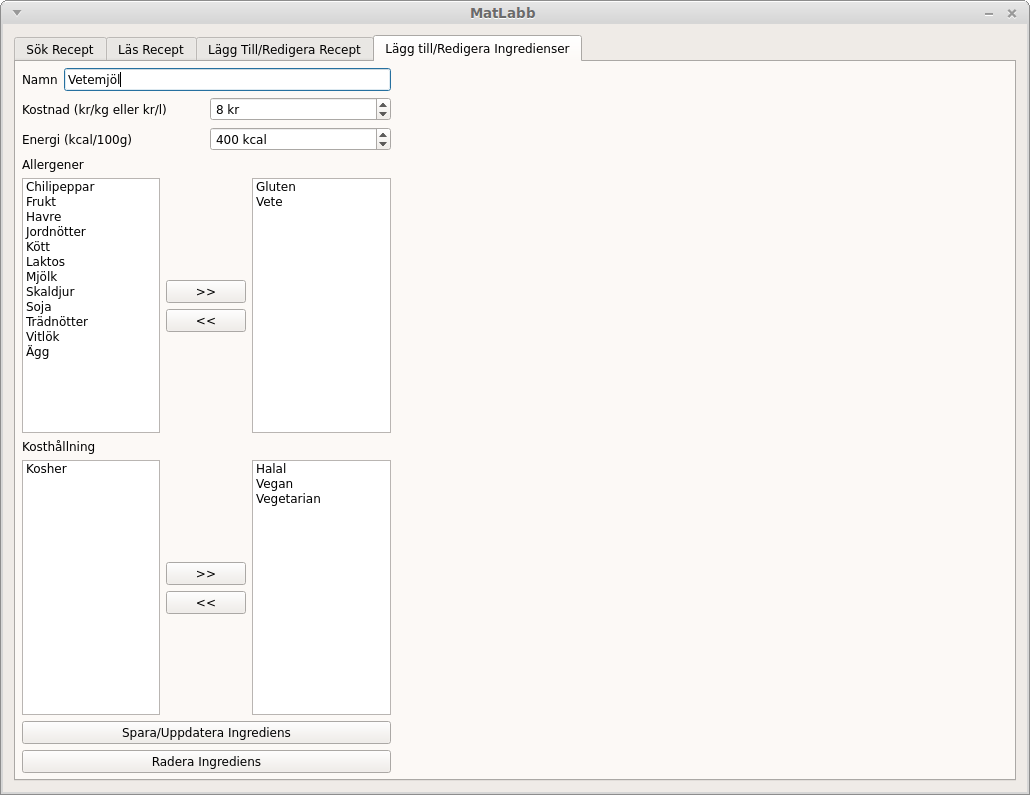
\includegraphics[scale=0.44]{lagg_till_ingrediens.png} 
        \caption{Lägg till/Redigera Ingrediens} 
        \label{fig:laggtillingrediensvyn}
\end{figure} 

Detta görs på följande vis, i godtyckligt ordning, förutom sista steget som måste ske sist. 

\begin{itemize}
\item Steg 1: Fyll i en titel i titelfältet.
\item Steg 2: Fyll i energiinehåll i energifältet.
\item Steg 3: Fyll i kostnad i kostnadsfältet. 
\item Steg 4: Markera de allergener, och klicka på knappen \verb+>>+ för att lägga till dem till ingrediensen. 
\item Steg 5: Markera de kosthållningar som man kan upprätthålla samtidigt som man äter din ingrediens. Lägg till dessa på samma sätt som allergener.
\item Steg 6: Klicka på \verb+Spara/Uppdatera Ingrediens+. Nu går ingrediensen att lägga till i recept och användas för att söka bland recept.
\end{itemize}


